\chapter{Tác động nhóm}

Tác động nhóm (Group Action) cho phép chúng ta đếm những cấu hình tổ hợp mà việc vét cạn rồi loại bỏ sẽ tốn nhiều công sức cũng như sai sót.

\section{Tác động nhóm}

Cho tập hợp $M$ và nhóm $G$. Ta nói $G$ \textit{tác động trái} lên $M$ với ánh xạ:
\[\alpha: G \times M \rightarrow M\]
thỏa mãn 2 tiên đề sau:

\begin{itemize}[noitemsep]
    \item Identity: $\alpha (e, m) = m$ với mọi $m \in M$
    \item Compatibility: $\alpha (g, \alpha (h, m)) = \alpha (g h, x)$
\end{itemize}

Ta thường ký hiệu $\alpha (g, m)$ bởi $g(m)$ hay thậm chí đơn giản hơn là $gm$. Ký hiệu $gm$ sẽ được sử dụng từ đây về sau.

Khi đó 2 tiên đề trên tương đương với:

\begin{itemize}[noitemsep]
    \item Identity: $e m = m$ với mọi $m \in M$
    \item Compatibility: $g(hm) = (gh)m$ với mọi $m \in M$ và $g, h \in G$
\end{itemize}

\begin{definition}[Stabilizer]
    (tạm dịch - \textit{nhóm con ổn đinh}). Với phần tử $m \in M$, tập hợp các phần tử $g \in G$ mà $gm = m$ được gọi là nhóm con ổn định của nhóm $G$. Ta ký hiệu
    \[G_m = \{ g \in G : gm = m \}\]
\end{definition}

\begin{definition}[Orbit]
    (tạm dịch - \textit{quỹ đạo}) của phần tử $m \in M$ là tập hợp
    \[G(m) = \{gm : g \in G\}\]
\end{definition}

\begin{remark}
    Hai orbit của hai phần tử bất kì hoặc rời nhau, hoặc trùng nhau.
\end{remark}

\begin{proof}
    Giả sử ta có $m_1, m_2 \in M$ mà $G(m_1) \cap G(m_2) \neq \emptyset$.

    Khi đó tồn tại $g_1, g_2 \in G$ để $g_1 m_1 = g_2 m_2$. Suy ra $m_1 = g_1^{-1} g_2 m_2$.

    Mà mọi phần tử trong $G(m_1)$ có dạng $g m_1$ nên $g m_1 = g g_1^{-1} g_2 m_2$ nên $G(m_1) \subseteq G(m_2)$.

    Chứng minh tương tự ta cũng có $G(m_2) \subseteq G(m_1)$ nên $G(m_1) \equiv G(m_2)$.
\end{proof}

\begin{corollary}
    Tập hợp $M$ là giao của các orbit rời nhau. Giả sử ta có $t$ orbit rời nhau $G(m_1), G(m_2), \ldots, G(m_t)$ thì
    \[M = G(m_1) \cup G(m_2) \cup \ldots \cup G(m_t)\]
\end{corollary}

\begin{example}
    Cho nhóm $\mathcal{S}_3$ có 6 phần tử $(1)(2)(3)$, $(1)(2,3)$, $(2)(1,3)$, $(3)(1,2)$, $(1,2,3)$, $(1,3,2)$.

    Xét tập hợp $M = \{1, 2, 3\}$. Khi đó, xét từng hoán vị trên, ta có:
    \[G_1 = \{(1)(2)(3), (1)(2,3)\}\]
    và
    \[G(1) = \{ 1, 2, 3 \}\]
\end{example}

Ta nhận thấy $G(1) = G(2) = G(3)$, và $\lvert G \rvert = 6 = \lvert G_1 \rvert \cdot \lvert G(1) \rvert$

Hay nói cách khác, $\lvert G(m) \rvert = [G: G_m]$ với $G_m$ là stabilizer của phần tử $m$ và $[G: G_m]$ là subgroup index của $G_m \subset G$, và bằng $\frac{\lvert G \rvert}{\lvert G_m \rvert}$ nếu là nhóm hữu hạn.

\begin{definition}
    Hai phần tử $m, n \in M$ được gọi là \textit{có quan hệ} với nhau dưới tác động của nhóm $G$ nếu tồn tại phần tử $g \in G$ sao cho $m = g n$.
    Ta ký hiệu là $m \tilde{G} n$.
\end{definition}

\begin{remark}
    Quan hệ được định nghĩa như trên là quan hệ tương đương.
\end{remark}

\begin{proof}
    Ta cần chứng minh quan hệ trên có tính phản xạ, đối xứng và bắc cầu.
    
    1. Tác động nhóm phải thỏa mãn $e m = m$ với mọi $m \in M$. Do đó có tính phản xạ.

    2. Với mọi $m, n$ mà $m \tilde{G} n$ thì tồn tại $g \in G$ mà $m = gn$. Do tồn tại $g^{-1} \in G$, nhân cho 2 vế ta có $g^{-1} m = n$, nghĩa là
    $n \tilde{G} m$. Vậy quan hệ này có tính đối xứng.

    3. Nếu $m \tilde{G} n$ và $n \tilde{G} p$ thì tồn tại 2 phần tử $g_1, g_2 \in G$ mà $m = g_1 n$ và $n = g_2 p$.
    Suy ra $m = g_1 g_2 p$, tương đương $m \tilde{G} p$, do đó có tính bắc cầu.
\end{proof}

\section{Bổ đề Burnside}

Các trạng thái khác nhau của tập hợp $M$ có thể là \textit{tương đương} nhau nếu chúng nằm trong cùng lớp tương đương dưới tác động của nhóm $G$.

Bổ đề Burnside cho phép chúng ta tính được số trạng thái khác nhau (hay cấu hình khác nhau) mà chúng ta dễ bị nhầm lẫn hoặc bỏ sót trong quá trình vét cạn.

\begin{lemma}[Bổ đề Burnside]
    Với nhóm $G$ tác động lên tập hợp $M$, ta có:
    \[t_G = \frac{1}{\lvert G \rvert} \sum_{g \in G} \lvert M^g \rvert \]
    trong đó, $t_G$ là số lớp tương đương của tập $M$ dưới tác động của nhóm $G$

    $\lvert M^g \rvert$ là số điểm bất động của tập $M$ dưới tác động của phần tử $g$, nghĩa là $M^g = \{ m \in M : gm = m\}$.
\end{lemma}

\section{Ví dụ bài toán đếm sử dụng bổ đề Burnside}

\begin{example}
    Cho hình tứ diện đều. Ta tô 4 đỉnh của nó bằng 3 màu xanh, đỏ, vàng. Hỏi có bao nhiêu cách tô như vậy?

    Ta cần lưu ý một điều, 2 cách tô là tương đương nhau (giống nhau) nếu tồn tại một phép quay các đỉnh biến cách tô này thành cách tô kia.

    \begin{figure}[ht]
        \centering
        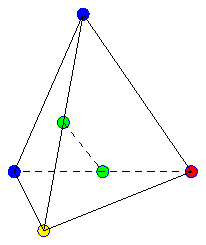
\includegraphics{pics/tetrahedron/tetrahedron1.pdf}
        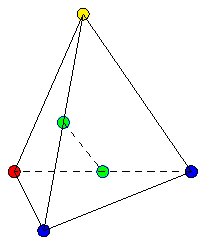
\includegraphics{pics/tetrahedron/tetrahedron2.pdf}
        \caption{Phép quay trục tạo bởi trung điểm hai cạnh đối nhau}
    \end{figure}

    Như hình trên ta thấy nếu chọn trục quay là đường thẳng nối trung điểm 2 cạnh đối diện (2 điểm xanh lá) thì đỉnh trên và đỉnh dưới đổi chỗ cho nhau (xanh và vàng), đỉnh trái và đỉnh phải đổi chỗ cho nhau (xanh và đỏ).

    Ta giải bài này như sau:

    Đầu tiên ta đánh số các đỉnh của tứ diện (như hình)

    \begin{figure}[ht!]
        \centering
        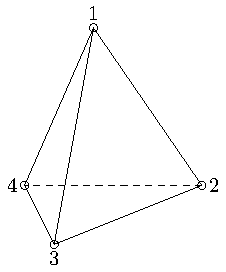
\includegraphics{pics/tetrahedron/tetrahedron3.pdf}
        \caption{Đánh số hình}
    \end{figure}
    
    Ta có 3 trường hợp biến đổi sau:

    \underline{Trường hợp 1}. Giữ nguyên 1 đỉnh và trục quay là đường thẳng đi qua đỉnh đó và tâm của mặt đối diện.

    \begin{figure}[ht!]
        \centering
        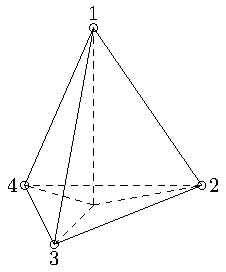
\includegraphics{pics/tetrahedron/tetrahedron4.pdf}
        \caption{Trường hợp 1}
    \end{figure}

    Khi đó phép quay (ngược chiều đồng hồ) tương ứng hoán vị $(1)(2,3,4)$ (quay 60 độ) và $(1)(2,4,3)$ (quay 120 độ).

    Do ta chọn 1 đỉnh cố định thì ta có 4 cách chọn, và với mỗi cách chọn đỉnh cố định ta có thể quay 2 cách nên ta có tổng là 8 hoán vị.

    \underline{Trường hợp 2}. Ta chọn trung điểm 2 cạnh đối nhau và nối lại thành trục quay như hình trong ví dụ. Khi đó tương ứng với hoán vị $(1,4)(2,3)$.

    Ta có $\frac{C^2_4}{2!} = 3$ hoán vị.

    \underline{Trường hợp 3}. Hoán vị đồng nhất $(1)(2)(3)(4)$.

    Tóm lại, tập hợp $M$ ở đây là tập hợp 4 đỉnh của tứ diện, và nhóm tác động lên $M$ là nhóm con 12 phần tử của $\mathcal{S}_4$.

    Như vậy, ví dụ với hoán vị $(1)(2,3,4)$, nếu ta muốn sau phép quay giữ nguyên trạng thái (hay nói cách khác là tìm $M^g$) thì ta
    tô màu đỉnh 1 tùy ý, đỉnh 2-3-4 chung màu (cũng tùy ý).

    Suy ra ta có $3 \cdot 3$ cách tô. Tương tự với các hoán vị dạng $(1,4)(2,3)$.

    Như vậy $t_G = \frac{1}{12}(1 \cdot 3^4 + 8 \cdot 3^2 + 3 \cdot 3^2) = 15$ cách tô màu khác nhau.
\end{example}

Tổng quát, nếu có $k$ màu thì số lớp tương đương là
\[t_G = \frac{1}{12}(1 \cdot k^4 + 8 \cdot k^2 + 3 \cdot k^2) = \frac{1}{12}(k^4 + 11 k^2)\]

\section{Chỉ số chu trình}

Với mỗi hoán vị trong tập $G$ (theo định lý Cayley thì mọi nhóm hữu hạn đều isomorphism với nhóm con nào đó của nhóm hoán vị), ta viết dưới dạng các chu trình độc lập
\[\underbrace{(g_1) (g_2) \ldots (g_{t_{1}})}_{t_1} \underbrace{(g_{j_1} g_{j_2}) (g_{j_3} g_{j_4})\ldots}_{t_2}\]
Nếu ta viết hoán vị dưới dạng các chu trình rời nhau, ta gọi

\begin{tabular}{c c}
    $t_1$ & là số chu trình có độ dài 1 \\
    $t_2$ & là số chu trình có độ dài 2 \\
    $\ldots$ & tương tự \\
    $t_n$ & là số chu trình có độ dài $n$
\end{tabular}

Khi đó, chỉ số chu trình của hoán vị ứng các biến $z_1, z_2, \ldots, z_n$ là
\[I_g (z_1, z_2, ,\ldots, z_n) = z_1^{t_1} z_2^{t_2} \ldots z_n^{t_n}\]

\begin{example}
Xét hoán vị $(1,2,3)(4)(5)(6,7) \in \mathcal{S}_7$

Ta có 2 chu trình độ dài 1, 1 chu trình độ dài 2 và 1 chu trình độ dài 3.
Không có chu trình độ dài 4, 5, 6, 7.

Do đó chỉ số chu trình là 
\[I_g (z_1, z_2, z_3) = z_1^2 z_2^1 z_3^1\]

\end{example}

\begin{remark}
    Bất kì hoán vị nào thuộc $\mathcal{S}_n$ đều thỏa $1 \cdot t_1 + 2 \cdot t_2 + \ldots + n \cdot t_n = n$.
\end{remark}

\begin{definition}[Cyclic index]
    (tạm dịch - \textit{chỉ số chu trình}) của nhóm G là
    \[P_G (z_1, z_2, \ldots, z_n) = \frac{1}{G}\sum_{g \in G} I_g (z_1, z_2, \ldots, z_n)\]
\end{definition}

Nhìn lại ví dụ về tứ diện bên trên, các đỉnh nằm trong cùng chu trình cần được tô cùng màu. Như vậy mỗi $z_i$ tương ứng với một màu.

Từ đó, với ví dụ trên
\[P_G(z_1, z_2, z_3) = \frac{1}{12}\big(z_1^4 + 8 z_1 z_3 + 3 z_2^2\big)\]

Cho mỗi $z_i = 3$ ta có kết quả phép tính theo bổ đề Burnside.

\section{Định lý Polya}

Định lý Polya là một mở rộng cho bổ đề Burnside, cho phép chúng ta đếm số lớp tương đương thỏa mãn điều kiện nhất định (về số lượng phần tử nhất định nhận trạng thái nhất định).

Ví dụ với hình tứ diện như trên nhưng ta thêm điều kiện tô 2 đỉnh màu vàng, 1 đỉnh màu đỏ và 1 đỉnh màu xanh (không tô tổng quát nữa).

Ta ký hiệu tập $R$ là tập hợp các trạng thái có thể nhận của mỗi phần tử $m \in M$.
\[R = \{r_1, r_2, \ldots, r_c \}\]
Ở ví dụ trên thì $R = \{\text{đỏ}, \text{xanh}, \text{vàng}\}$.

Ta thay mỗi $z_i$ trong chỉ số chu trình bằng tổng $\sum_{r \in R} r^i$.

\begin{example}
    Giả sử ta tô màu 4 đỉnh tứ diện với 2 màu $R = \{r_1, r_2\}$.

    Với $z_1$ ta thay bằng $r_1 + r_2$

    Với $z_2$ ta thay bằng $r_1^2 + r_2^2$

    Với $z_3$ ta thay bằng $r_1^3 + r_2^3$

    Khi đó $P_G$ tương đương với
    \[\frac{1}{12}\big[(r_1 + r_2)^4 + 8 \cdot (r_1 + r_2)(r_1^3 + r_2^3) + 3 \cdot (r_1^2 + r_2^2)^2\big]\]
    Khai triển ra (lưu ý là ở đây không có tính giao hoán phép nhân)
    \begin{align*}
        (r_1 + r_2)^4 = & r_1 r_1 r_1 r_1 + r_1 r_1 r_1 r_2 + r_1 r_1 r_2 r_1 + r_1 r_1 r_2 r_2 \\
        + & r_1 r_2 r_1 r_1 + r_1 r_2 r_1 r_2 + r_1 r_2 r_2 r_1 + r_1 r_2 r_2 r_2 \\
        + & r_2 r_1 r_1 r_1 + r_2 r_1 r_1 r_2 + r_2 r_1 r_2 r_1 + r_2 r_1 r_2 r_2 \\
        + & r_2 r_2 r_1 r_1 + r_2 r_2 r_1 r_2 + r_2 r_2 r_2 r_1 + r_2 r_2 r_2 r_2
    \end{align*}

    Mình thấy rằng có 16 cấu hình khác nhau tương ứng 16 cách tô 2 màu cho 4 đỉnh. Tương tự

    \begin{align*}
        (r_1 + r_2) (r_1^3 + r_2^3) & = r_1^4 + r_1 r_2^3 + r_2 r_1^3 + r_2^4 \\
        & = r_1 r_1 r_1 r_1 + r_1 r_2 r_2 r_2 + r_2 r_1 r_1 r_1 + r_2 r_2 r_2 r_2
    \end{align*}

    và cuối cùng

    \begin{align*}
        (r_1^2 + r_2^2)^2 & = r_1^4 + r_1^2 r_2^2 + r_2^2 r_1^2 + r_2^4 \\
        & = r_1 r_1 r_1 r_1 + r_1 r_1 r_2 r_2 + r_2 r_2 r_1 r_1 + r_2 r_2 r_2 r_2
    \end{align*}

    Việc không có tính giao hoán với phép nhân làm biểu thức cồng kềnh và phức tạp.
    Do đó mình thêm một tập hợp $W$ là vành giao hoán, và xét ánh xạ $w: R \mapsto W$ với $w(r_i) = w_i$.

    Khi đó nếu thay $r_i$ bởi $w_i$ vào bên trên biểu thức sẽ rất đẹp
    \[P_G(w_1, w_2) = \frac{1}{12} \big[(w_1 + w_2)^4 + 8 (w_1 + w_2) (w_1^3 + w_2^3) + 3 (w_1^2 + w_2^2)^2\big]\]

    Khai triển và thu gọn ta có
    \begin{align*}
    P_G(w_1, w_2) & = \frac{1}{12} \big[12 w_1^4 + 12 w_1^3 w_2 + 12 w_1^2 w_2^2 + 12 w_1 w_2^3 + 12 w_2^4\big] \\
    & = w_1^4 + w_1^3 w_2 + w_1^2 w_2^2 + w_1 w_2^3 + w_2^4
    \end{align*}

    Ở đây, định lý Polya nói rằng, số mũ của $w_i$ thể hiện số lượng phần tử của tập $M$ nhận giá trị $r_i$,
    và hệ số trước mỗi toán hạng là số lớp tương đương tương ứng với số lượng phần tử của tập $M$ nhận các giá trị $r_i$.

    Nói cách khác:
    \begin{itemize}[noitemsep]
        \item có 1 lớp tương đương mà 4 đỉnh nhận màu $r_1$
        \item có 1 lớp tương đương mà 3 đỉnh nhận màu $r_1$ và 1 đỉnh nhận màu $r_2$
        \item có 1 lớp tương đương mà 2 đỉnh nhận màu $r_1$ và 2 đỉnh nhận màu $r_2$
        \item có 1 lớp tương đương mà 1 đỉnh nhận màu $r_1$ và 3 đỉnh nhận màu $r_2$
        \item cuối cùng là 1 lớp tương đương mà 4 đỉnh nhận màu $r_2$.
    \end{itemize}
\end{example}

Quay lại vấn đề tô 4 đỉnh tứ diện với 3 màu xanh, đỏ, vàng. Tìm số cách tô 2 đỉnh màu vàng, 1 đỉnh màu đỏ và 1 đỉnh màu xanh.

Đặt $w(\text{vàng}) = x$, $w(\text{đỏ}) = y$ và $w(\text{xanh}) = z$

Ta có
\[P_G = \frac{1}{12} \big[(x + y + z)^4 + 8 \cdot (x + y + z) (x^3 + y^3 + z^3) + 3 \cdot (x^2 + y^2 + z^2)^2\big]\]

Như vậy đề bài tương ứng việc tìm hệ số của hạng tử $x^2 yz$ trong biểu thức trên. Mình tính ra kết quả là 1.